\documentclass{article}
\usepackage{amssymb}
\usepackage{mathtools}
\usepackage{amsmath}
\usepackage{hyperref}
\usepackage{setspace}
\usepackage[utf8]{inputenc}
 
\usepackage{listings}
\usepackage{color}
\usepackage{graphicx}
\usepackage[english]{babel}
 
\setlength{\parindent}{4em}
\setlength{\parskip}{1em}
 
\definecolor{codegreen}{rgb}{0,0.6,0}
\definecolor{codegray}{rgb}{0.5,0.5,0.5}
\definecolor{codepurple}{rgb}{0.58,0,0.82}
\definecolor{backcolour}{rgb}{0.95,0.95,0.92}
 
\lstdefinestyle{mystyle}{
    backgroundcolor=\color{backcolour},   
    commentstyle=\color{codegreen},
    keywordstyle=\color{magenta},
    numberstyle=\tiny\color{codegray},
    stringstyle=\color{codepurple},
    basicstyle=\footnotesize,
    breakatwhitespace=false,         
    breaklines=true,                 
    captionpos=b,                    
    keepspaces=true,                 
    numbers=left,                    
    numbersep=5pt,                  
    showspaces=false,                
    showstringspaces=false,
    showtabs=false,                  
    tabsize=2
}

\newcommand{\norm}[1]{\left\lVert#1\right\rVert}
 
\lstset{style=mystyle}

\everymath{\displaystyle}

\begin{document}

\raggedright

\doublespacing


\title{ {\Huge{Data Mining 2015 - Homework 4}} }
\author {Ludovico Fabbri 1197400}
\maketitle


\section{Problem 1}
Here we will compute the PageRank in a special case and we will prove a rule.

\subsection{}
Compute the PageRank scores of the nodes of the following two graphs, for teleporting prob- ability equal to zero (i.e., $\beta = 1$), using the equations of the stationary distribution. Take advantage of the symmetries to reduce the number of unknown variables: are there nodes that we know a priori that they have the same PageRank score?

\newpage

\begin{figure} [h]
\centering
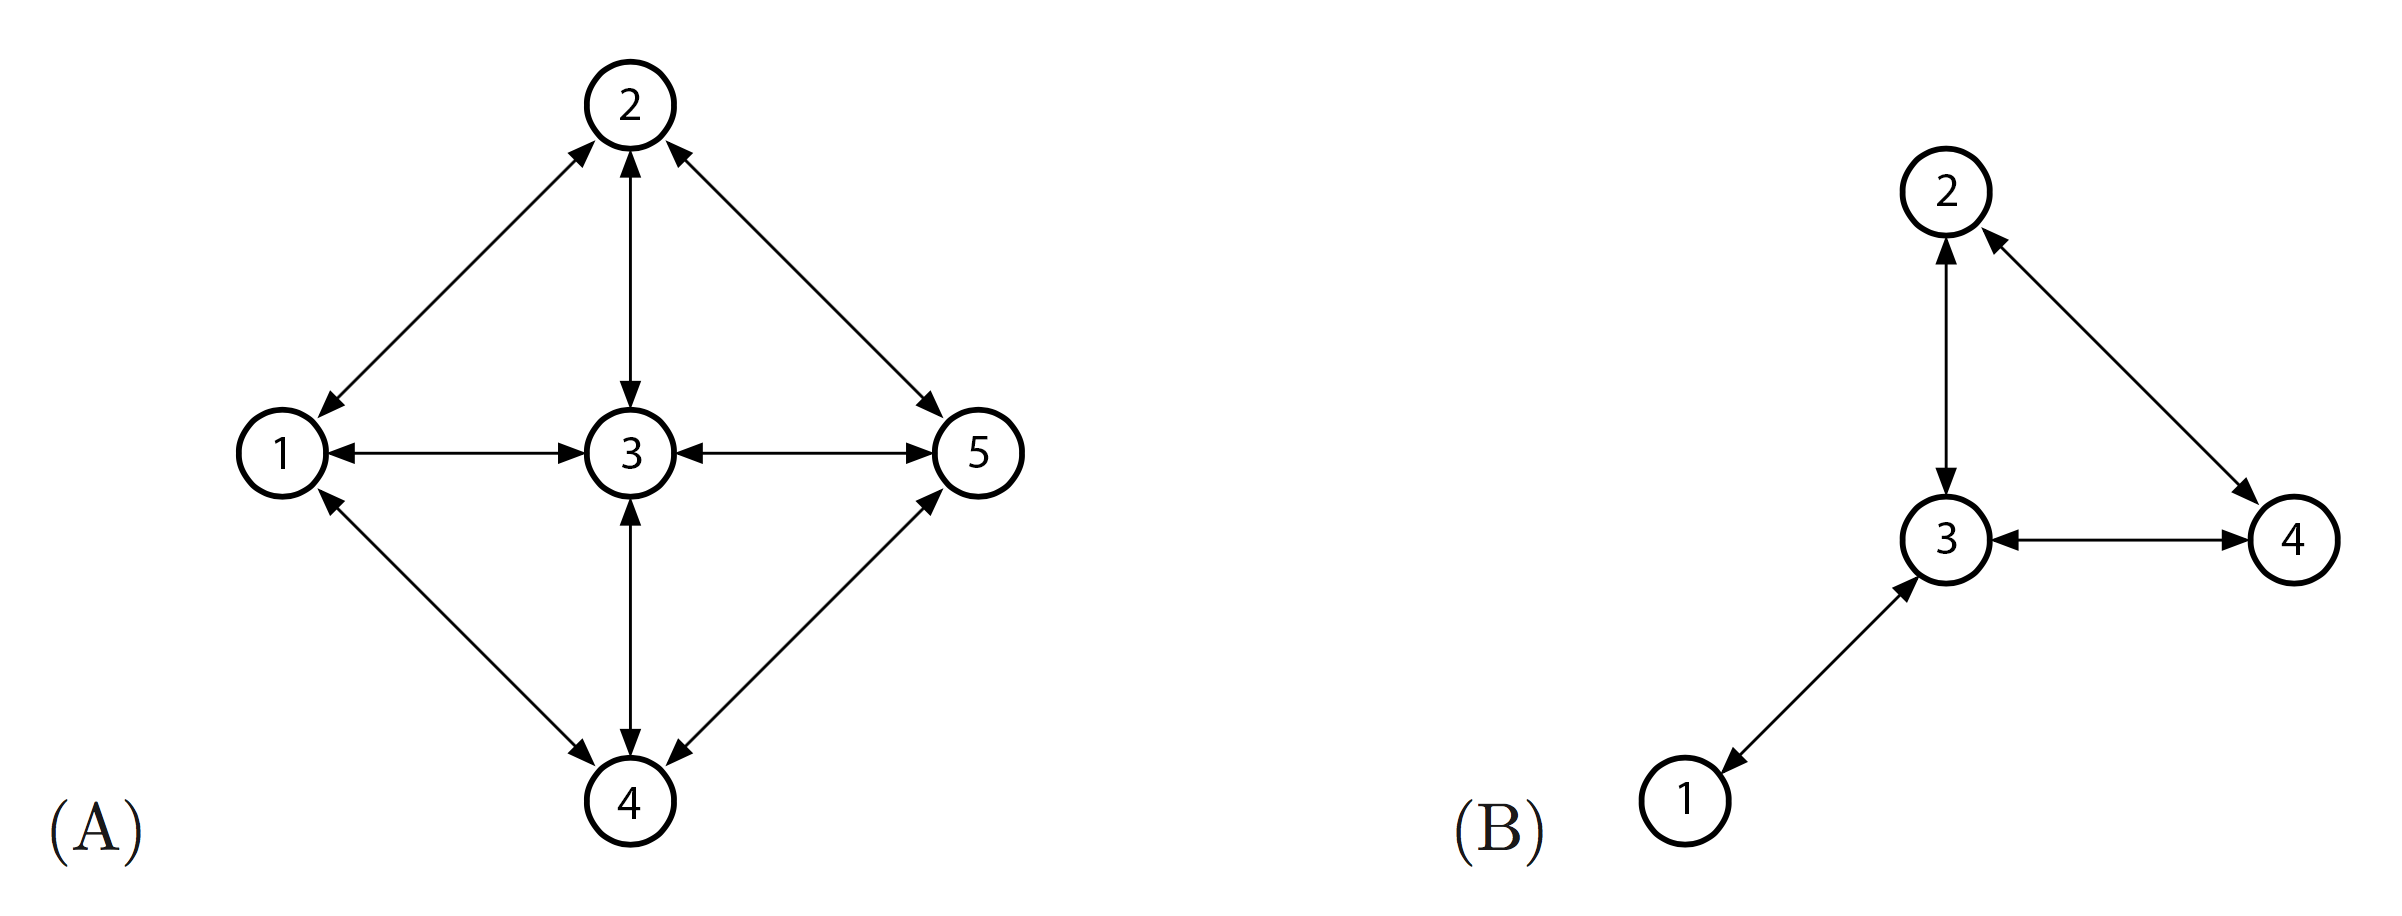
\includegraphics[width=120mm]{graphs}
\caption{graphs  \label{graphs}}
\end{figure}

In the figure above we can see the index assigned for each node of the graphs.


Now we can define the transition matrix P for both the graphs, where each row is the probability vector for the respective node of the graph (in each row the sum of the transition probabilities must be equal to 1):

\begin{equation} \label{eq:matriceTransizione1}
P_{1} =
\begin{bmatrix}
    0 & \frac{1}{3} & \frac{1}{3} &	\frac{1}{3}	& 0  \\
    \frac{1}{3} & 0 & \frac{1}{3} &	0 & \frac{1}{3}	 \\
   \frac{1}{4} & \frac{1}{4} & 0 &	\frac{1}{4}	& \frac{1}{4}  \\
       \frac{1}{3} & 0 & \frac{1}{3} &	0 & \frac{1}{3}	 \\
        0 & \frac{1}{3} & \frac{1}{3} &	\frac{1}{3}	& 0  \\
\end{bmatrix}
\end{equation}

\begin{equation} \label{eq:matriceTransizione2}
P_{2} =
\begin{bmatrix}
    0 & 0 & 1 & 0  \\
    0 & 0 & \frac{1}{2} & \frac{1}{2}  \\
   \frac{1}{3} & \frac{1}{3} & 0 &  \frac{1}{3}  \\
        0 & \frac{1}{2} & \frac{1}{2} & 0  \\
\end{bmatrix}
\end{equation}

With $\beta = 1$ we have no teleporting (so the graph must be connected otherwise the pagerank will never converge, as it is in this case), to calculate the pagerank for each node of the graphs we can use the stationary distribution equation:

$$\pi = \pi \cdot P$$ 

From this equation we can obtain a system of linear equations and resolve it using Kramer or other methods. Since $\pi$ is a probability distribution we have also to add the constraint that 
$$ \sum_{i=1}^{n} \pi_{i} = 1 $$
where n is the number of the states (nodes of the graph).

Thus for the first graph we have that the pagerank vector and the system of linear equations are respectively:

$$
\pi_{1} = \left[ x_{1} \; x_{2} \; x_{3} \; x_{4} \; x_{5} \right]
$$

$$
S_{1} = \pi_{1} \cdot P_{1} = 
\begin{cases}{l}
\frac{1}{3}x_{2} + \frac{1}{4}x_{3} + \frac{1}{3}x_{4}  =   x_{1}   \\
\frac{1}{3}x_{1} + \frac{1}{4}x_{3} + \frac{1}{3}x_{5}  =   x_{2}   \\
\frac{1}{3}x_{1} + \frac{1}{3}x_{2} + \frac{1}{3}x_{4} + \frac{1}{3}x_{5}  =   x_{3}  \\
\frac{1}{3}x_{1} + \frac{1}{4}x_{3} + \frac{1}{3}x_{5}  =   x_{4}   \\
\frac{1}{3}x_{2} + \frac{1}{4}x_{3} + \frac{1}{3}x_{4}  =   x_{5}   \\
x_{1} + x_{2} + x_{3} + x_{4} + x_{5} = 1
\end{cases}
$$

The solution of the linear system gives the pagerank vector for the first graph:

$$\pi_{1} = \left[ \frac{3}{16} \; \frac{3}{16} \; \frac{4}{16} \; \frac{3}{16} \; \frac{3}{16} \; \right]$$


For the second graph we have that the pagerank vector and the system of linear equations are respectively:

$$
\pi_{2} = \left[ x_{1} \; x_{2} \; x_{3} \; x_{4} \; x_{5} \right]
$$

$$
S_{2} = \pi_{2} \cdot P_{2} =
\begin{cases}{l}
\frac{1}{3}x_{3}  =   x_{1}   \\
\frac{1}{3}x_{3} + \frac{1}{2}x_{4}  =   x_{2}   \\
x_{1} + \frac{1}{2}x_{2} + \frac{1}{2}x_{4} =  x_{3}  \\
\frac{1}{2}x_{2} + \frac{1}{3}x_{3}  =   x_{4}   \\
x_{1} + x_{2} + x_{3} + x_{4}  = 1
\end{cases}
$$


The solution of the linear system gives the pagerank vector for the second graph:


$$\pi_{2} = \left[ \frac{1}{8} \; \frac{1}{4} \; \frac{3}{8} \; \frac{1}{4} \right]$$


Now, to answere the question ```are there nodes that we know a priori that they have the same PageRank score?'' intuively we can say that two nodes that have the same neighbours will have also the same pagerank; in the case of graph A we have for example nodes 1 and 5 that have the same neighbours (2, 3, 4) and nodes 2 and 4 that have also the same neighbours (1, 3, 5), for graph B we have nodes 2 and 4 that have in common the node 3 as neighbour.

More formally we can say that two nodes that have the same probability vector in the transition matrix P will have also the same pagerank.




\subsection{}
Notice that here we have a special case: All the edges are bidirectional and we have $\beta$ = 1. After observing the scores of the nodes that you computed in these examples, make a conjecture about the PageRank score of a node in this special case, and prove it.


A stationary distribution $\pi$ is:

\begin{equation}\label{eq:stationary1}
\pi(x) = \sum_{n} \pi(n) P(n,x)          
\end{equation}

foreach node x in the graph, where n is the generic neighbour node of v and $P(n,x)$ is the probability of the transition from node n to node v.

Or equivalently:

$$
\pi = \pi P
$$

From the results of the pageranks computed in the previous point we can make this conjecture: ``for an undirected and connected graph G (not bipartite) the random walk on G converge to a stationary distribution $\pi=\frac{d(x)}{2|E|}$ '', where d(x) is the number of incident edges in the node x (degree) and $|E|$ is the number of edges in the graph.

To proove the correctness of this conjecture, let's say $N(x)$ is the set of neighbours of the node x. From the definition of stationary distribution (\ref{eq:stationary1}) we can write:

$$
\pi(x) = \sum_{n \in N(x)} \frac{d(n)}{2|E|} \cdot \frac{1}{d(n)} = \sum_{n \in N(x)} \frac{1}{2|E|} = \frac{d(x)}{2|E|}
$$

where $\frac{d(n)}{2|E|}$ is the pagerank of the node n and $\frac{1}{d(n)}$ is the transition probability from node n to node x. We can ask: is this valid for every node? We know that for a stationary distribution we have the costrain $\sum_{n \in N} \pi(n) = 1$. Let's see if this is valid:

$$
\sum_{n \in N} \frac{d(n)}{2|E|} = \frac{2|E|}{2|E|} = 1
$$

In fact $\sum_{n \in N} d(n) = 2|E|$ is correct since in an undirected graph each edge is counted twice in the sum. This finally prooves that our original conjecture was correct.








\section{Problem 2}
In class we saw an algorithm for estimating the second moment in a stream. Here we will see another method and we will implement it.
We have a universe $U = {e_1, . . . , e_l}$ of l elements. Assume that the stream that arrives is the $s = (s_1,s_2,...,s_n)$,
where each $s_j \in U$ and $\forall e_i \in U$ let $m(e_i)$ be the number of times that $e_i$ appears in s: $m(e_i) =  { j ; s_j = e_i } $.
Let $Y = (Y_1, Y_2, Y_l)$ be a random vector, where each $Y_i$ is a random value in $\left\{ -1, 1 \right\}$, each with probability $\frac{1}{2}$, all $Y_{is}$ being mutually independent.
Define

$$ X = \sum_{i}^{l} Y_{i} \cdot m(e_i) $$


\subsection{Part 1.1}

\begin{itemize}
    \item Compute $E[X]$ and $E[X^2]$ \\
\end{itemize}


For the linearity of the expectation we can bring out the sum and write:

$$
E[X] = \sum_{i}^l E[Y_i \cdot m(e_i)]
$$

$m(e_i)$ is a costant, so we can bring it out of the expectation as well (always for the linearity property):

$$
E[X] = \sum_{i}^l m(e_i) \cdot E[Y_i]
$$

Now let's compute the expectation of $Y_i$:

$$
E[Y_i] = \sum_{i \in \left\{-1, 1 \right\}} i \cdot Pr(Y_i = i) = -\frac{1}{2} + \frac{1}{2} = 0
$$

So in the end:

$$
E[X] = \sum_{i}^l m(e_i) \cdot 0 = 0
$$


Now let's compute $E\left[ X^2 \right]$:


$$
E[X^2] = E \left[ \sum_{i=1}^l Y_i \cdot m(e_i) \right]^2
$$

We can rewrite it as following:

$$
E[X^2] = E \left[ \sum_{i=1}^l Y_i \cdot m(e_i)  \cdot  \sum_{j=1}^l Y_j \cdot m(e_j)    \right]
$$

The expression inside the expectation is simply a square of a polynomial, we can split it in two sums:

$$
\left[ \sum_{i=1}^l Y_i \cdot m(e_i)  \cdot  \sum_{j=1}^l Y_j \cdot m(e_j)    \right] =
\sum_{i=1, j=1, i=j}^l Y_i Y_j \cdot m(e_i) m(e_j) \; \; + 2\sum_{i=1, j=1, i \neq j}^l Y_i Y_j \cdot m(e_i) m(e_j)
$$


where the sum on the right is the sum of the squares of the elements of the polynomial and the second sum is the sum of the double products between the elements of the polynomial.

Now to compute the expectation of the first sum we can use again the linearity of the expecation as we did in the previous point:

$$
E \left[ \sum_{i=1, j=1, i=j}^l Y_i Y_j \cdot m(e_i) m(e_j) \right] =
\sum_{i=1, j=1, i=j} E[Y_i Y_j] \cdot m(e_i) m(e_j) = 
$$
$$
\sum_{i=1}^l E[Y_i^2] \cdot m^2(e_i)
$$

Now we can observe that:

$$
E[Y_i^2] = 1^2 \cdot \frac{1}{2} + (-1)^2 \cdot \frac{1}{2} = 1
$$


so the previous expression becomes:

$$
E \left[ \sum_{i=1, j=1, i=j}^l Y_i Y_j \cdot m(e_i) m(e_j) \right] =
\sum_{i=1}^l m^2(e_i)
$$

Now let's compute the expectation of the second sum:

$$
E\left[ 2\sum_{i=1, j=1, i \neq j}^l Y_i Y_j \cdot m(e_i) m(e_j) \right] = 
$$
$$
2\sum_{i=1, j=1, i \neq j}^l E[Y_i Y_j] \cdot m(e_i) m(e_j) 
$$

Because $Y_i$ and $Y_j$ are independent random variables we can write:

$$
2\sum_{i=1, j=1, i \neq j}^l E[Y_i Y_j] \cdot m(e_i) m(e_j) = 
2\sum_{i=1, j=1, i \neq j}^l E[Y_i] \cdot E[Y_j] \cdot m(e_i) m(e_j) 
$$

From the previous point we know that $E[Y_i] = 0$ and $E[Y_j] = 0$, so  we find that:

$$
E\left[ 2\sum_{i=1, j=1, i \neq j}^l Y_i Y_j \cdot m(e_i) m(e_j) \right] = 0
$$


So in the end we found that:

$$
E[X^2] = \sum_{i=1}^l m^2(e_i)
$$


which is the second moment of the stream.






\subsection{Part 1.2}

\begin{itemize}
    \item Use the above idea to propose an algorithm for estimating the second moment of stream s.
\end{itemize}

From what we have found above, we can think of an algorithm that gives a good estimate of the second moment while processing a stream.
We found that the expected value of the square of $ X = \sum_{i}^{l} Y_{i} \cdot m(e_i) $ is exactly the second moment, so we can think to use $X^2$ as an estimate of the second moment as well. Since a single estimate is not really useful because it could be close to the expected value but also not so close, we are going to use many of them through a family of hash functions. So before the algorithm start we initialize a family of k hash functions and a vector of length k where in each cell we mantain a counter. For each data coming from the stream we hash a string key representing the data to an integer for every hash function of the family, and if the hash number is even we add $+1$ in the relative counter in the vector, otherwise we add $-1$. This last operation is done as representing the random variables $Y_i$, but it is more efficient in space since we have not to store the entire $Y$ vector; because we are using hash functions, we know that a property of an hash function is that the hash of the same element will give always the same result, so we know that for a given key the same hash function will awlays update the counter in the same way ($+1$ or $-1$).
To compute the estimate of the second moment we take all the squares of the counters in the vector and take the mean. Below there is a python class that implement this algorithm, which i will use in the next point to compute an estimate of the second moment for the twitter stream. The algorithm compute three distinct estimates of the second moment using respectively 100, 1000 and 10000 hash functions.

\clearpage


\begin{lstlisting}
from helpers import *

class SecondMomentOnline:

    def __init__(self):
        self.k = 10000  # number of used hash functions
        self.counts = [0 for i in range (self.k)]
        self.hashFunctions = [hashFamily(i) for i in range(self.k)]
        self.estimates = {}




    def updateCounts(self, username):
        i = 0
        for hasher in self.hashFunctions:
            hash = hasher(username)
            #print hash
            if hash % 2 == 0:
                self.counts[i] += 1
            else:
                self.counts[i] -= 1
            i += 1

    def clear(self):
        self.counts = [0 for k in range (self.k)]
        self.estimate = -1



    def computeEstimate(self):
        temp = 0
        i = 0
        for c in self.counts:
            if (i == 100):
                self.estimates[100] = temp / 100
            if (i == 1000):
                self.estimates[1000] = temp / 1000
            temp += c**2
            i += 1
        temp = temp / self.k
        self.estimates[self.k] = temp

\end{lstlisting}









\subsection{Part 2}
Source code is in the ``src'' folder. 

\begin{itemize}
    \item \textit{TwitterStream.py}: implement a class responsible to establish a stream with Twitter using OAuth1.0 protocol, accepting only tweets geolocalized in Rome
    \item \textit{SecondMomentOffline.py}: implement a class responsible to compute the second moment on file
    \item \textit{SecondMomentOnline.py}: implement a class responsible to compute an estimate of the second moment online on a stream. For the accuracy i choose to compute three estimates using respectively 100, 1000, and 10000 hash functions. 
    \item \textit{helpers.py}: implement a method to generate a family of hash functions that hash to integers
    \item \textit{program.py}: the executable program file
    \item \textit{tweets.txt}: text file for storing tweets coming from stream data
\end{itemize}

Below a table showing the results. On the left there is the time stamp in seconds, then there are the estimates of the second moment respectively using 100, 1000 and 10000 hash functions, and in the last column there is the exact value of the second moment computed offline.          

\begin{center}
  \begin{tabular}{ | c || c | c | c || c |}
    \hline
    (t) & k=100 & k=1000 & k=10000 & offline \\ \hline
    152 & 91 & 76 & 75 & 74 \\ \hline
    309 & 320 & 302 & 309 & 303 \\ \hline
    time3 \\
    \hline
  \end{tabular}
\end{center}










\end{document}


